\documentclass{article}

\usepackage{latexsym}

\usepackage{amsmath}
\usepackage{amssymb}
\usepackage{amsthm}

\usepackage{graphicx}

\usepackage{tikz}
\usepackage[top=1in,bottom=1in,right=1in,left=1in]{geometry}

\newtheorem{theorem}{Theorem}[section]

\begin{document}
\title{Descartes' Circle Theorem}
\author{Dave Neary}

\maketitle

\section{Statement of theorem}

Descartes' Circle Theorem relates to the relationship between packed "kissing" circles -
that is, groups of circles that are mutually tangent to each other. The modern form of
the theorem (slightly different from the statement of Descartes) states that, given 3
pairwise tangent circles, there are two circles that are tangent to all of the circles
(see figure \ref{fig:apollonian_circles}).

Defining the curvature $c$ of a circle as the inverse of its radius, and setting the
curvature of a circle which is surrounding the 3 other circles to be negative, the
curvatures of four circles which are all mutually tangent to each other satisfy 
the relation:

\[ 2(c_1^2 + c_2^2 + c_3^2 + c_4^2) = (c_1 + c_2 + c_3 + c_4)^2 \]

\begin{figure}[htb]
        \center{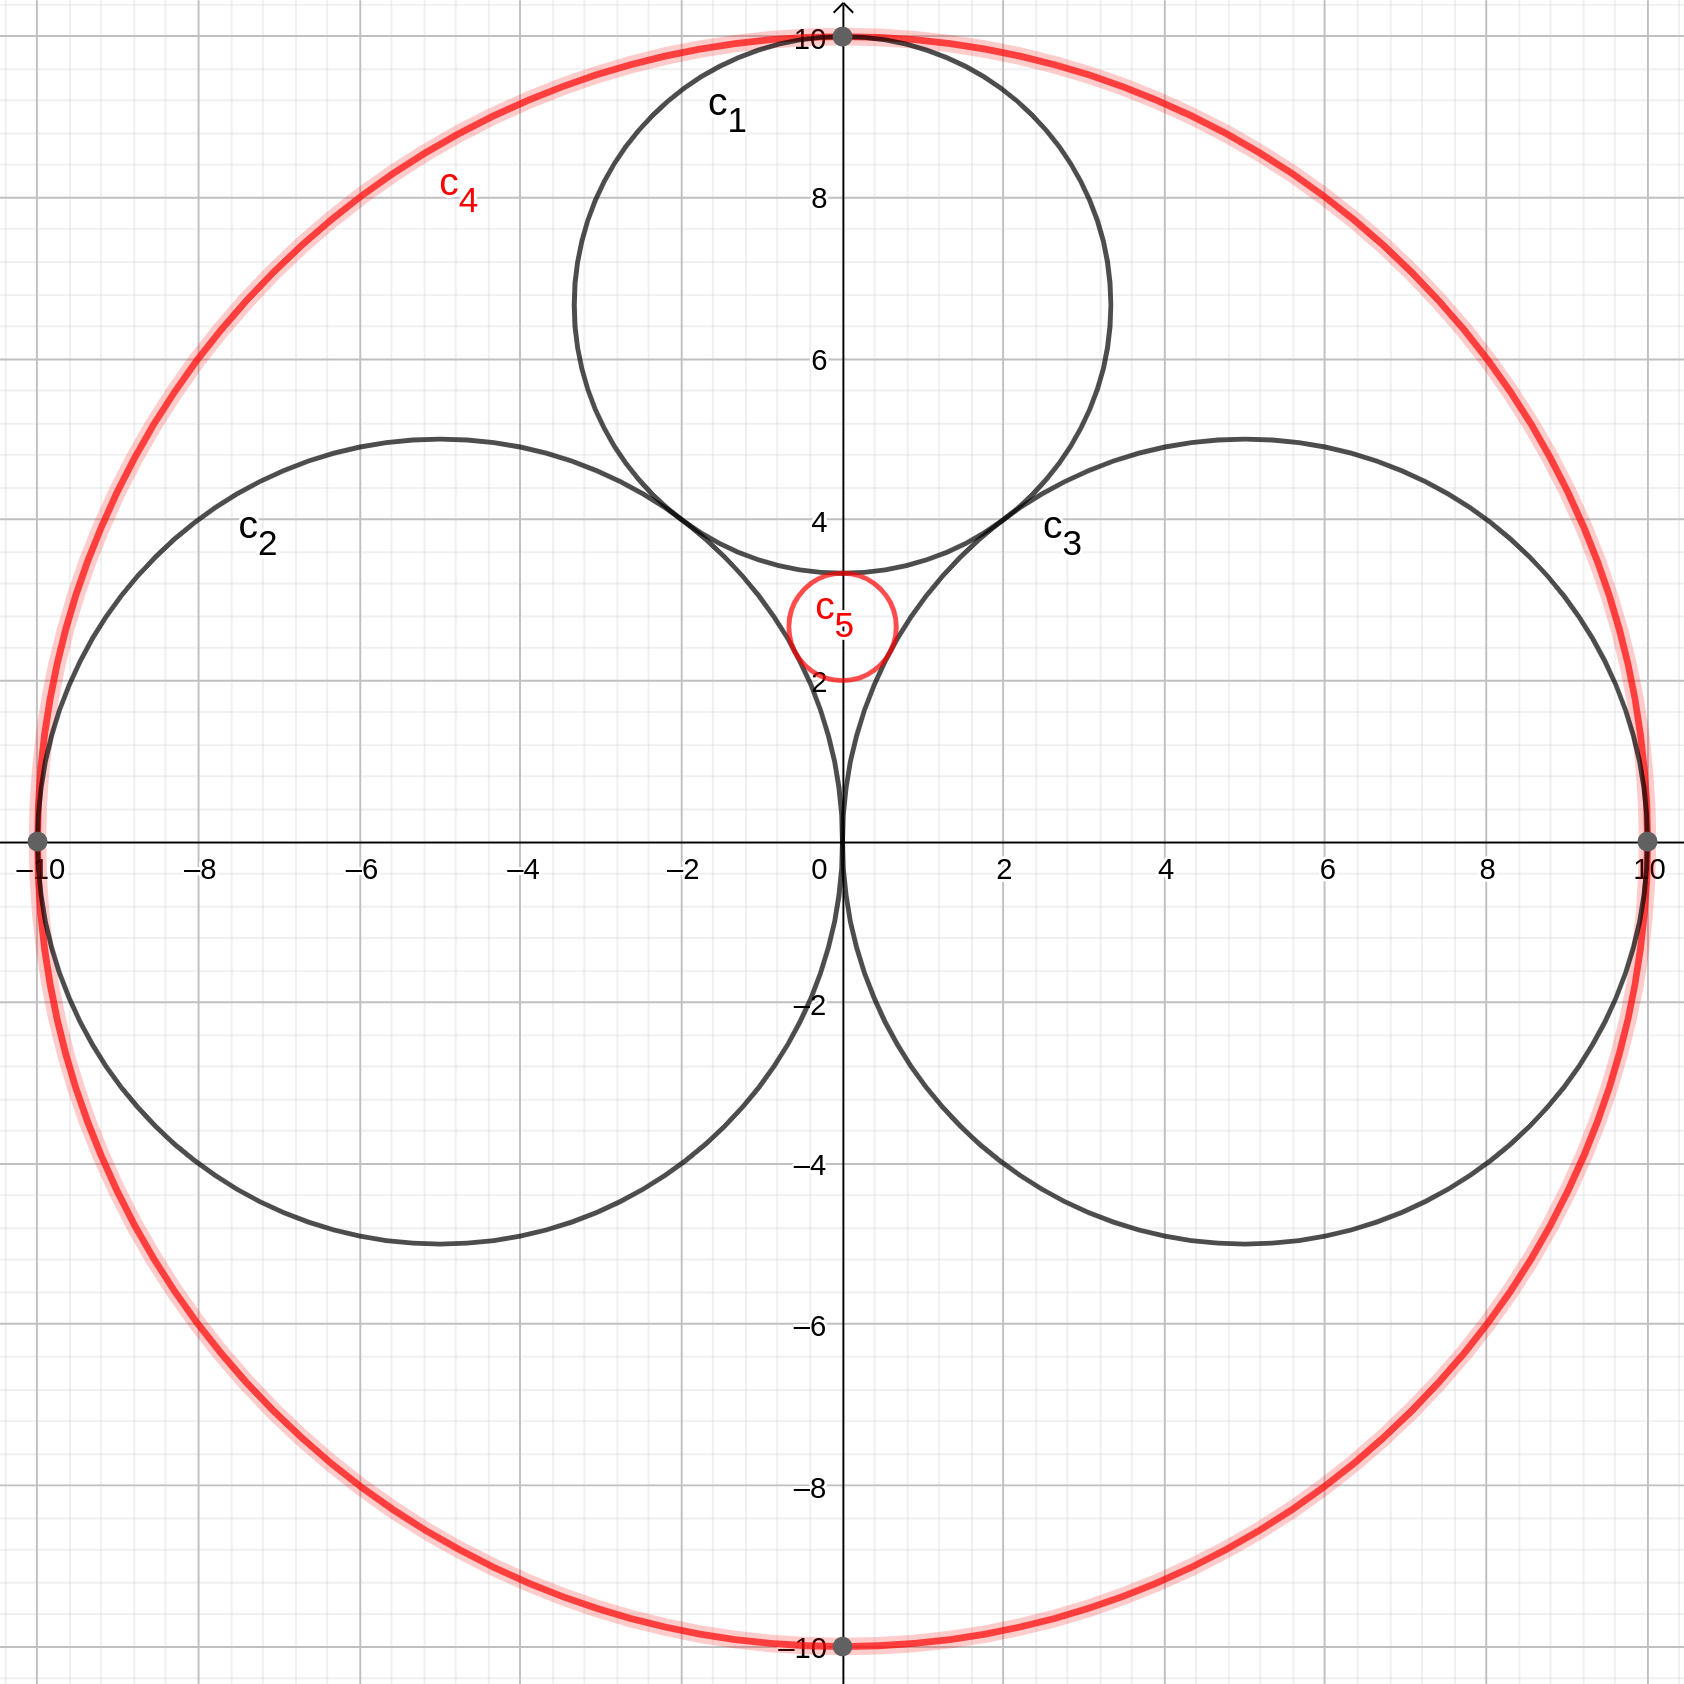
\includegraphics[width=0.5 \linewidth]{apollonian_circles.png}}
        \caption{Two circles $c_4$ and $c_5$ are mutually tangent to $c_1, c_2, c_3$}
        \label{fig:apollonian_circles}
\end{figure}

This paper is a presentation of a proof of this theorem which uses circle inversion.

\section{Circle inversion}

Circle inversion is an involution (that is, a function which is also its own inverse) 
of the plane. A circle $C$ with center $O$ and radius $r$ maps a point $P$ to a point $P'$
such that $P$, and $P'$ are both on a ray with endpoint $O$ and:
\[ |OP|\cdot |OP'| = r^2 \]

This maps points on the circle $C$ to themselves, and maps points inside the circle to
points outside the circle, and vice versa.

\begin{tikzpicture}[scale=5.3,cap=round,>=latex]

        % draw the unit circle
        \draw[thick] (0cm,0cm) circle(1cm);
        % draw a ray from (0,0) to (1.2,1.6)
	\draw[thick] (0,0) -- (1.6, 1.2);

	% draw a red point at (0,0)
	\draw[fill=red] (0,0) circle(0.1mm);
	% draw a blue point at (2/5, 3/10)
	\draw[fill=blue] (0.4,0.3) circle(0.1mm);
	% draw a blue point at (21/25,28/25)
	\draw[fill=blue] (1.6,1.2) circle(0.1mm);

	% label points O, P, P'
	\draw (0,0) node[left=1pt] {$O$}
	      (0.4,0.3) node[left=1pt] {$P$}
	      (1.6,1.2) node[left=1pt] {$P'$};

	% label the lengths of |OP|, |OP'|
	\draw (0.16, 0.12) node[right=3pt] {$|OP| = \frac{1}{2}$}
	      (1.2, 0.9) node[right=3pt] {$|OP'| = 2$};

\end{tikzpicture}

Where things start to get very interesting is when we start to look at inversions of
circles and lines.

\begin{itemize}
	\item A circle inside the circle of inversion maps to a circle outside, and vice versa.
	\item A circle straddling the circle of inversion will map to another circle sharing the
		intersection points with the circle of inversion.
	\item The diameter of a circle coincident with the ray through the center of the circle of
		inversion inverts to the diameter of the circle it maps to. (note: circle centers
		do \textbf{not} invert to the centers of the circles they invert to).
	\item Lines which do not go through the center of the circle of inversion invert to circles
		which go through the center of the circle of inversion, and vice versa.
	\item Lines through the center of the circle of inversion invert to themselves.
\end{itemize}

\end{document}
